\documentclass[10 pt,usenames,dvipsnames, oneside]{article}
\usepackage{../../../modelo-ensino-medio}



\begin{document}

\begin{center}
  \begin{minipage}[l]{3cm}

\includegraphics[width=2cm]{logo}    
\end{minipage}\hfill
\begin{minipage}[r]{.8\textwidth}
 {\Large \scshape Atividade: O problema dos bodes}  
\end{minipage}
\end{center}
\vspace{.2cm}

\ifdefined\prof
%Habilidades da BNCC
\begin{objetivos}
\item a
\end{objetivos}

%Caixa do Para o Professor
\begin{goals}
%Objetivos específicos

\begin{enumerate}
\item Calcular a probabilidade de um evento considerando duas estratégias distintas.
\end{enumerate}

\tcblower

%Orientações e sugestões
Nesta atividades as interpretações clássica e frequentista podem ser usadas. De fato, a noção frequentista de probabilidade é usada muitas vezes para validar a suposição de equiprobabilidade de eventos elementares. Este problema gerou muita polêmica nos anos 1990 do século XX e é conhecido como problema de Monty Hall (incluir referência). Neste link é possível visualizar uma simulação do problema. (incluir link)

Uma sugestão para lidar com esta atividade é realizar a simulação do programa de televisão em sala de aula. Peça a turma para se dividir em dois grupos: um que adotará a estratégia de nunca trocar a escolha inicial e, o outro, de sempre trocar. A cada simulação do jogo deverá ser registrado, em dada grupo, se houve vitória ou derrota. Esta simulação pode ser feita com três cartas de versos idênticos, por exemplo. Sugere-se repetir a simulação pelo menos 30 vezes em cada grupo. No final compare com os alunos a frequência de vitórias em cada grupo e depois discuta sobre a melhor estratégia.

Caso esteja disponível internet e projetor, neste \href{https://www.geogebra.org/m/Ec9xubPJ}{link} será possível simular várias partidas do jogo e ir registrando os resultados em cada equipe.
\end{goals}

\bigskip
\begin{center}
{\large \scshape Atividade}
\end{center}
\fi

Em um programa de televisão semanal, um jogo oferece como prêmio um automóvel a um espectador escolhido da plateia. O candidato a ganhar o automóvel é convidado pelo apresentador do programa a escolher uma entre três portas idênticas, atrás das quais há um carro em uma delas e, nas outras duas, há um bode em cada uma.

\begin{figure}[H]
\centering

\noindent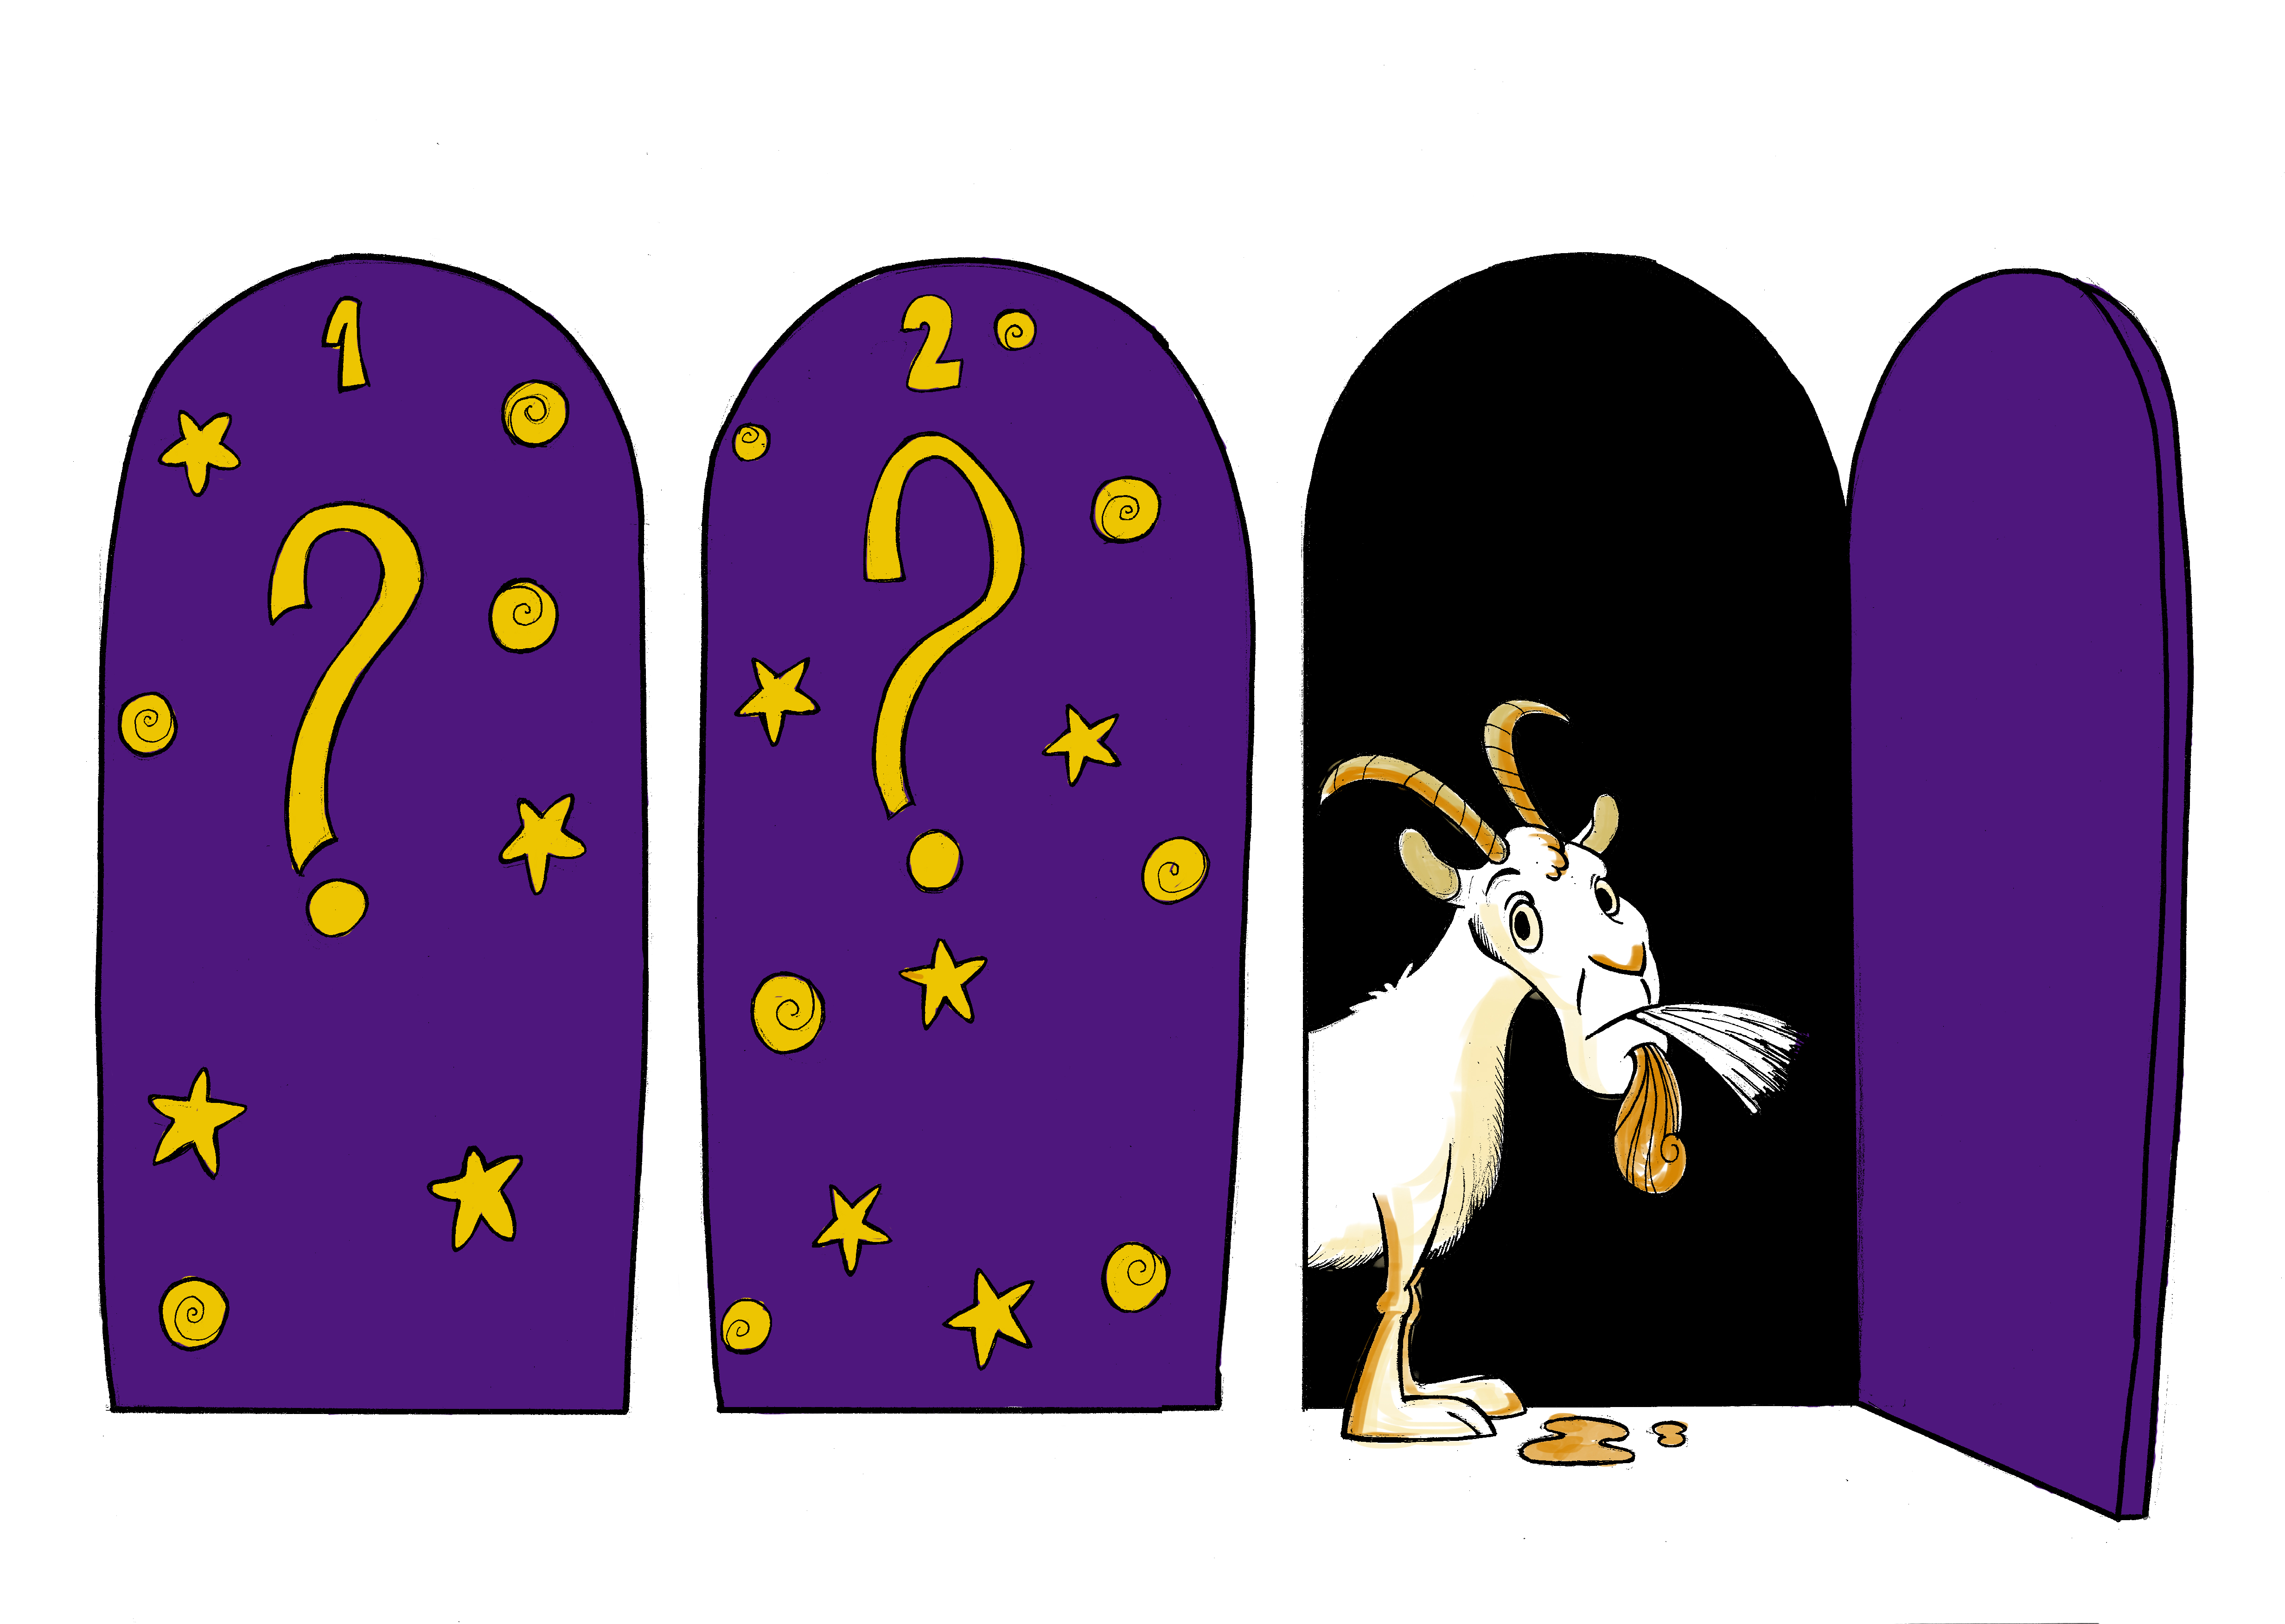
\includegraphics[width=250bp]{bode}
\caption{Problema dos bodes}
\end{figure}


Depois de o candidato escolher a porta, o apresentador, que sabe o que tem atrás de cada uma delas, abre uma das portas não escolhidas, mostrando que atrás dela tem um bode. Então, o apresentador oferece ao candidato decidir entre manter sua escolha inicial ou trocar de porta.

Qual deve ser a melhor estratégia para o candidato (trocar ou não trocar de porta) de modo que a sua probabilidade de ganhar o automóvel seja a maior possível?

\ifdefined\prof
\begin{solucao}

A melhor estratégia será trocar de porta. Observe que inicialmente, o candidato tem probabilidade $1/3$ de escolher a porta com o carro e $2/3$ de escolher uma porta com um bode. Assim, se a estratégia do candidato for manter a escolha inicial, sua chance de ganhar o carro será $1/3$.

Por outro lado, se a estratégia do candidato for trocar de porta, sua chance de ganhar o carro será $\frac{2}{3}$: se ele escolher a porta que tem o carro (com probabilidade $\frac{1}{3}$) e trocar de porta ele não ganhará. No entanto se ele escolher uma porta com bode (cuja probabilidade é $\frac{2}{3}$) e trocar de porta, ele ganhará. Logo, sob a estratégia “trocar de porta”, a probabilidade de ganhar o carro é $\frac{2}{3}$.

Veja neste \href{https://www.geogebra.org/m/Ec9xubPJ}{link} uma simulação deste problema

\end{solucao}
\fi

\end{document}